

\tikzset{every picture/.style={line width=0.75pt}} %set default line width to 0.75pt        

\begin{tikzpicture}[x=0.75pt,y=0.75pt,yscale=-1,xscale=1]
	%uncomment if require: \path (0,265); %set diagram left start at 0, and has height of 265
	
	%Shape: Ellipse [id:dp7551326114257342] 
	\draw   (75.79,147.86) .. controls (81.98,142.31) and (103.89,156.65) .. (124.72,179.88) .. controls (145.54,203.12) and (157.41,226.46) .. (151.21,232.01) .. controls (145.02,237.56) and (123.11,223.23) .. (102.28,199.99) .. controls (81.46,176.75) and (69.59,153.42) .. (75.79,147.86) -- cycle ;
	%Shape: Ellipse [id:dp03803498476554046] 
	\draw   (151.21,232.01) .. controls (143.32,229.37) and (148.16,193.64) .. (162.02,152.21) .. controls (175.87,110.77) and (193.5,79.32) .. (201.39,81.95) .. controls (209.28,84.59) and (204.44,120.32) .. (190.59,161.76) .. controls (176.73,203.2) and (159.1,234.65) .. (151.21,232.01) -- cycle ;
	%Shape: Ellipse [id:dp25139516998021827] 
	\draw   (151.21,232.01) .. controls (147.46,224.59) and (167.65,206.82) .. (196.31,192.33) .. controls (224.97,177.84) and (251.25,172.11) .. (255.01,179.53) .. controls (258.76,186.96) and (238.57,204.72) .. (209.9,219.21) .. controls (181.24,233.71) and (154.96,239.43) .. (151.21,232.01) -- cycle ;
	%Shape: Ellipse [id:dp5445438337062236] 
	\draw   (201.39,81.95) .. controls (208.68,77.95) and (226.57,96.51) .. (241.36,123.41) .. controls (256.14,150.31) and (262.21,175.36) .. (254.92,179.37) .. controls (247.63,183.37) and (229.74,164.82) .. (214.96,137.92) .. controls (200.17,111.01) and (194.1,85.96) .. (201.39,81.95) -- cycle ;
	%Shape: Ellipse [id:dp17386590304939553] 
	\draw   (75.79,147.86) .. controls (67.88,145.22) and (67.77,124.19) .. (75.56,100.91) .. controls (83.35,77.62) and (96.08,60.88) .. (103.99,63.53) .. controls (111.9,66.18) and (112.01,87.2) .. (104.22,110.49) .. controls (96.43,133.78) and (83.7,150.51) .. (75.79,147.86) -- cycle ;
	%Shape: Ellipse [id:dp2638569941795088] 
	\draw   (103.54,64.32) .. controls (105.32,56.19) and (128.49,54.36) .. (155.29,60.23) .. controls (182.09,66.1) and (202.38,77.44) .. (200.6,85.57) .. controls (198.82,93.7) and (175.65,95.53) .. (148.85,89.66) .. controls (122.05,83.79) and (101.77,72.45) .. (103.54,64.32) -- cycle ;
	
	%Image [id:dp4637388297623295] 
	\draw (449.85,149.94) node  {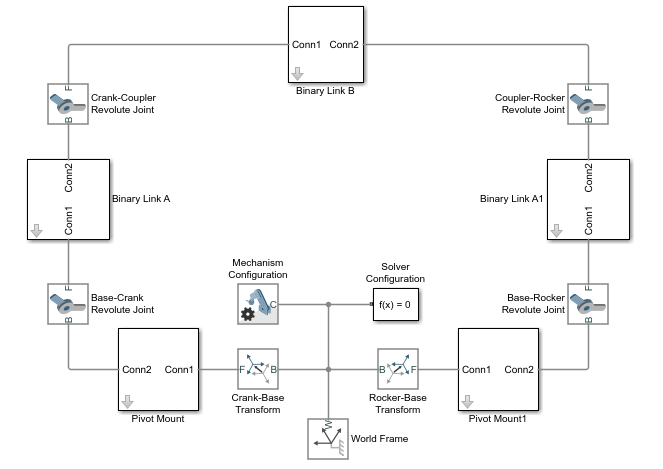
\includegraphics[width=218.28pt,height=154.41pt]{simscape-close-loop.png}};
	%Image [id:dp5015666519585665] 
	\draw (449.17,127.32) node  {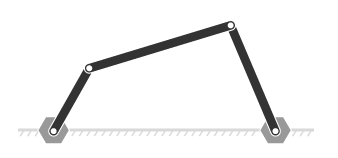
\includegraphics[width=85.25pt,height=39.85pt]{simscape-ex-closedloop.png}};
	%Shape: Ellipse [id:dp9896253160830154] 
	\draw  [color={rgb, 255:red, 255; green, 0; blue, 0 }  ,draw opacity=1 ] (389,69.94) .. controls (389,53.96) and (416.53,41) .. (450.5,41) .. controls (484.47,41) and (512,53.96) .. (512,69.94) .. controls (512,85.92) and (484.47,98.88) .. (450.5,98.88) .. controls (416.53,98.88) and (389,85.92) .. (389,69.94) -- cycle ;
	
	% Text Node
	\draw (103.56,164.12) node [anchor=north west][inner sep=0.75pt]  [rotate=-50.29] [align=left] {Link 1};
	% Text Node
	\draw (186.57,204.8) node [anchor=north west][inner sep=0.75pt]  [rotate=-333.98] [align=left] {Link 3};
	% Text Node
	\draw (73.68,120.6) node [anchor=north west][inner sep=0.75pt]  [rotate=-296.79] [align=left] {Link 3};
	% Text Node
	\draw (96,243) node [anchor=north west][inner sep=0.75pt]   [align=left] {Inertial coordinate};
	% Text Node
	\draw (115.9,58.87) node [anchor=north west][inner sep=0.75pt]  [rotate=-13.17] [align=left] {End effector};
	% Text Node
	\draw (159.34,177.84) node [anchor=north west][inner sep=0.75pt]  [rotate=-288.75] [align=left] {Link 2};
	% Text Node
	\draw (226.74,113.17) node [anchor=north west][inner sep=0.75pt]  [rotate=-61.48] [align=left] {Link 4};
	% Text Node
	\draw (64,32) node [anchor=north west][inner sep=0.75pt]   [align=left] {closed loop kinematic chain};
	% Text Node
	\draw (306,11) node [anchor=north west][inner sep=0.75pt]   [align=left] {"Which ensures that the connection is valid?};
	
	
\end{tikzpicture}